\section{Blokové schéma}
    Pro pohodlné použití je hlavní část zařízení soustředěna do jedné krabičky napájené přívodním síťovým kabelem. Uživatel pak dle potřeby zapojí zařízení využívající \qty{230}{V} a veškeré další periferie připojí za pomoci jednoho z vlastních konektorů. O stavu zařízení pak bude informován sérií notifikačních LED a malým displayem. Pro ilustraci je na obr.~\ref{fig:obrazky-hydros-control} uveden jeden z produktů řady HYDROS, který zvolil podobnou koncepci.


    \begin{figure}[h!]
        \centering
        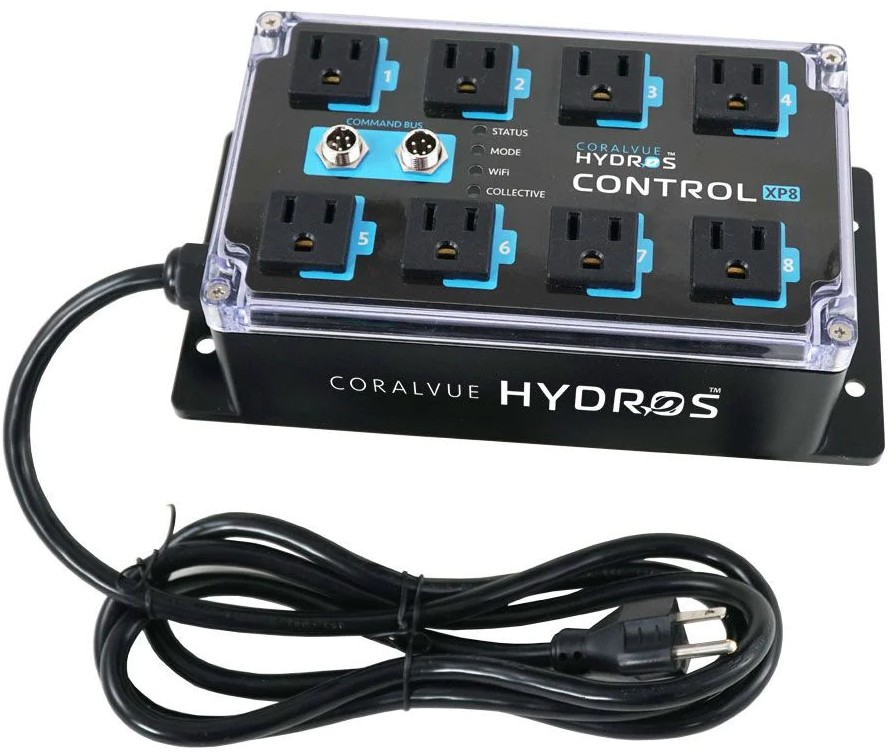
\includegraphics[width=0.8\textwidth]{obrazky/hydros.jpg}
        \caption{Ilustrační obrázek pro vzhled zařízení. CoralVue HYDROS Control XP8~\cite{coralvuehydros}. }
        \label{fig:obrazky-hydros-control}
    \end{figure}

    Blokové schéma zařízení se nachází na obr.~\ref{fig:blokove-schema}, podrobnějšímu popisu jednotlivých bloků se pak věnuje kapitola~\ref{kap:navrh-dilnich-bloku}. 
    
    Z hlediska bezpečnosti je potřeba zajistit, aby se uživatel ani samotná nízkonapěťová část obvodu nemohli dostat do kontaktu s nebezpečným napětím. Toho bude dosaženo galvanickým oddělením částí zařízení pracujících se síťovým napětím. V blokovém schématu (obr.~\ref{fig:blokove-schema}) jsou všechny tyto části podbarveny šedou barvou. Galvanického oddělení bude zajištěno použitím vhodných komerčně dostupných modulů, které již mají tento problém vyřešen. U relé modulu je potřeba zvolit variantu s optočlenem a pro napájecí zdroj s výstupem \qty{24}{V} pak zkontrolovat v dokumentaci přítomnost galvanického oddělení. 
    
    % Blokove schema
    \begin{figure}[h!]
        \centering
        \begin{tikzpicture}[
            node distance=2cm,
            blok/.style={draw, rectangle, rounded corners=8pt, minimum height=1.5cm, minimum width=3cm},
            rect/.style={draw, dashed, blue, inner sep=15pt, fit=#1},
            label/.style={blue}
        ]
            % barvičky
            \definecolor{barva-silove}{RGB}{220, 220, 220}
            \definecolor{barva-ridici}{RGB}{241, 196, 15}
        
            \node (napajeni) [blok, fill=barva-silove] {Napájecí zdroj 24V};
            \node (ridici) [blok, below of = napajeni, align=center, fill=barva-ridici] {Řídící jednotka \\ (ESP32)};
            \node (rele) [blok, right=0.5 of ridici, fill=barva-silove] {Relé modul};
            \node (zasuvky) [blok, right=0.5 of rele, fill=barva-silove] {Zásuvky 230VAC};
            \node (uzel) [style={draw, circle, minimum size=0.1cm, fill}, above=1cm of zasuvky] {};
            \node (sit) [blok, above= of uzel, fill=barva-silove ] {Přívod 230VAC};
            \node (display) [blok, below left=-0.5cm and 0.65cm of ridici] {Status display};
            \node (ledstrip) [blok, above left=-0.5cm and 0.65cm of ridici] {Status LED pásek};

            \node (konektor1) [blok, align=center, below left=1.5cm and -1.2cm of ridici] {Konektor pro periferie \\ \#1};
            \node (konektor2) [blok, align=center, below right=1.5cm and -1.2cm of ridici] {Konektor pro periferie \\ \#2};

            % Periferie
            \node (per1-1) [blok, align=center, below=1.2cm of konektor1] {Periferie \\ \#1.1};
            \node (per1-x) [blok, align=center, below=1.4cm of per1-1] {Periferie \\ \#1.X};
        
            \node (per2-1) [blok, align=center, below=1.2cm of konektor2] {Periferie \\ \#2.1};
            \node (per2-y) [blok, align=center, below=1.4cm of per2-1] {Periferie \\ \#2.Y};

            % Popisek
            \node (vlastovka) [font=\fontsize{35}{14}\selectfont, yscale=4,  above right=-5.2cm and 0.6cm of per2-1] {\}}; 

            \node (popisek1) [right=0cm of vlastovka,yshift=1cm, align=left] {Připojení senzorů: \\ -- teploměr \\ -- výška hladiny \\ -- pH \\ -- ...};
            \node (popisek2) [below=1cm of popisek1.south west, anchor=south west, align=left] {Řízení LED svícení};
            \node (popisek3) [below=1cm of popisek2.south west, anchor=south west, align=left] {...};

            % Spojovací linie
            \draw[-] (sit) -- (uzel);
            \draw[-] (uzel) -- (napajeni);
            \draw[-] (uzel) -- (zasuvky);
            \draw[-] (napajeni) -- (ridici);
            \draw[-] (ridici) -- (napajeni);
            \draw[-] (ridici) -- (display);
            \draw[-] (ridici) -- (ledstrip);
            \draw[-] (ridici) -- (konektor1);
            \draw[-] (ridici) -- (konektor2);
            \draw[-] (ridici) -- (rele);
            \draw[-] (rele) -- (zasuvky);
 
            \draw[-] (konektor1) -- (per1-1);
            \draw[dashed] (per1-1) -- (per1-x);
            
            \draw[-] (konektor2) -- (per2-1);
            \draw[dashed] (per2-1) -- (per2-y);
            
        
            % Obdélník, který obklopí vybrané uzly
            \node (hlavni-cast) [rect={(napajeni) (display) (ledstrip) (konektor1) (zasuvky)}] {};
            \node[label,above left=0.2cm and -3.6cm of hlavni-cast] {Hlavní šasi zařízení};
        \end{tikzpicture}
        
        \caption{Blokové schéma systému.}
        \label{fig:blokove-schema}
    \end{figure}
    

    
    

